\apendice{Documentación de usuario}

El presente apéndice constituye el manual de usuario final del sistema SugAIr. Su propósito principal es guiar al paciente o usuario a través de la interfaz móvil, explicando los requisitos técnicos necesarios para ejecutar el prototipo, el proceso de instalación en un entorno de pruebas y las instrucciones de uso para interactuar correctamente con el asistente virtual de nutrición.

\section{Introducción}
SugAIr se ha diseñado con un enfoque centrado en la accesibilidad y la simplicidad, adoptando el paradigma visual de las aplicaciones de mensajería instantánea tradicionales. Al ocultar la complejidad técnica del procesamiento de Inteligencia Artificial y la comunicación en red, el usuario final solo necesita interactuar con una interfaz de chat intuitiva para obtener asistencia nutricional especializada en diabetes.

\section{Requisitos de usuarios}
Para garantizar el correcto funcionamiento del prototipo en su estado actual de desarrollo, el usuario debe disponer de un entorno que cumpla con los siguientes requisitos técnicos y de permisos:

\begin{itemize}
    \item \textbf{Hardware:} Un dispositivo móvil inteligente (\textit{smartphone}) con sistema operativo Android o iOS.
    \item \textbf{Conectividad:} Conexión activa a la misma red de área local (Wi-Fi) en la que se encuentra desplegado el servidor principal del sistema.
    \item \textbf{Software de terceros:} La aplicación gratuita \textit{Expo Go} instalada en el dispositivo móvil.
    \item \textbf{Permisos del sistema:} Concesión explícita de permisos de acceso a la galería multimedia del dispositivo para permitir la selección y envío de etiquetas nutricionales o fotografías de alimentos.
\end{itemize}

\clearpage
\section{Instalación}

\begin{figure}
    \centering
    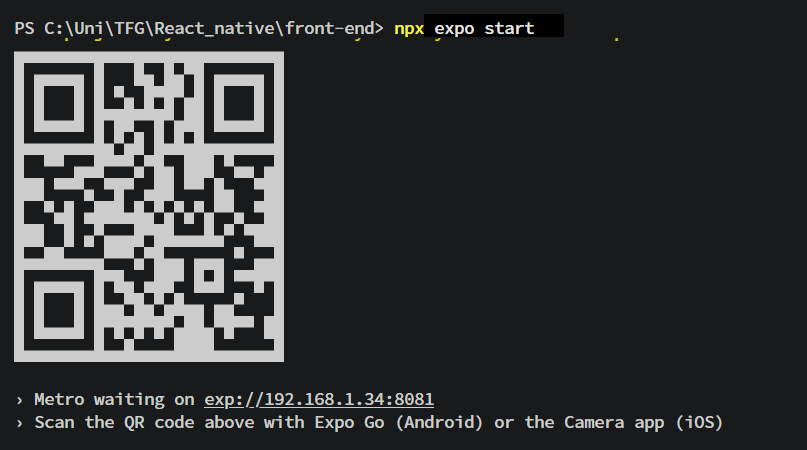
\includegraphics[width=0.5\linewidth]{QR.png}
    \caption{QR para abir con Expo Go}
    \label{fig:QR}
\end{figure}
Al tratarse de una prueba de concepto enmarcada en un Trabajo de Fin de Grado, la aplicación no se encuentra distribuida mediante las tiendas de aplicaciones comerciales (Google Play Store o Apple App Store). El despliegue en el terminal del usuario se realiza mediante sincronización local siguiendo estos pasos:

\begin{enumerate}
    \item Descargar e instalar la aplicación \textbf{Expo Go} desde la tienda oficial correspondiente al sistema operativo del dispositivo móvil.
    \item Asegurarse de que el dispositivo móvil está conectado a la misma red Wi-Fi que el dispositivo que aloja el servidor de SugAIr.
    \item Solicitar al administrador del sistema (el desarrollador) que inicie el entorno de ejecución, el cual generará un código QR en la pantalla del ordenador.
    \item Abrir la aplicación Expo Go en el dispositivo móvil y seleccionar la opción \textit{Scan QR Code}.
    \item Enfocar el código QR. La aplicación descargará el paquete de JavaScript, compilará la interfaz y ejecutará SugAIr automáticamente de forma nativa.
\end{enumerate}

Se podría ejecutar todo en el móvil, pero tendría que ser un dispositivo potente y con bastante RAM. Sería instalar Termux o algún terminal para Android, e instalar Go y Ollama para ejecutar los comandos de la guía del manual del programador


\section{Manual del usuario}
Una vez ejecutada la aplicación, el usuario interactuará con una única pantalla principal que centraliza todas las funcionalidades del asistente médico. El flujo de uso básico se divide en las siguientes acciones:

\subsection*{1. Interfaz principal y mensajería de texto}
\begin{figure}
    \centering
    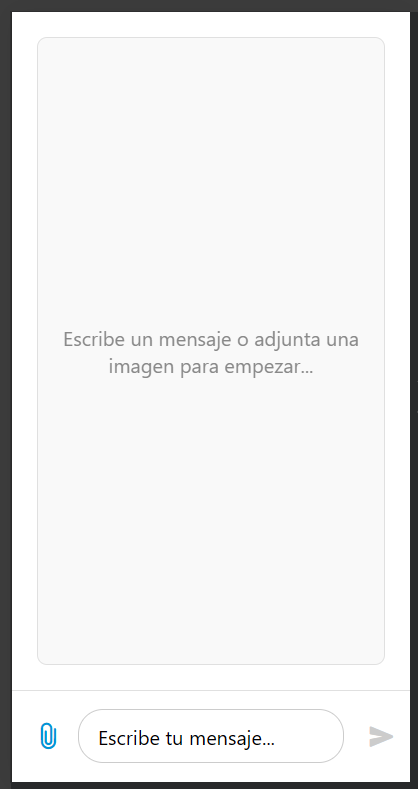
\includegraphics[width=0.9\linewidth]{al_abrir.png}
    \caption{Pantalla de inicio}
    \label{fig:al_abrir}
\end{figure}
Al abrir SugAIr, la pantalla mostrará un lienzo en blanco o un mensaje de bienvenida como la de la imagen \ref{fig:al_abrir}. En la parte inferior, anclada sobre el teclado virtual, se encuentra la barra de interacción.
Para realizar una consulta escrita estándar:
\begin{itemize}
    \item Pulsar sobre el cajón de texto que indica \textit{"Escribe tu mensaje..."}.
    \item Redactar la consulta deseada.
    \item Pulsar el botón azul con el icono de enviar (flecha) situado en el extremo derecho.
\end{itemize}

\subsection*{2. Análisis visual de alimentos, graficas de actividad física e información nutricional}
La característica principal del sistema es su capacidad multimodal. Para que la IA analice una fotografía de una etiqueta nutricional o un alimento o una gráfica de actividad física:
\begin{figure}
    \centering
    
\includegraphics[width=0.20\linewidth]{clip.png}
    \caption{Botón clip de adjuntar imágenes}
    \label{fig:clip}
\end{figure}
\begin{itemize}
    \item Pulsar el botón con el icono de un \textbf{clip} \ref{fig:clip} (adjuntar), situado a la izquierda de la barra de texto.
    \item El sistema operativo abrirá la galería de imágenes. El usuario debe seleccionar la fotografía deseada.
    \item Una vez seleccionada, aparecerá una pequeña imagen de previsualización justo encima de la barra de texto.
    \item Si el usuario se ha equivocado de imagen, puede descartarla pulsando el icono circular rojo con una cruz situado en la esquina de la miniatura.
    \item Para enviar la imagen a análisis, se debe pulsar el botón azul de enviar. Opcionalmente, se puede añadir texto explicativo en el cajón de mensajería antes de realizar el envío.
\end{itemize}

\subsection*{3. Espera y recepción de resultados}
Dado que el análisis de imágenes mediante Inteligencia Artificial requiere capacidad de cómputo, el procesamiento no es instantáneo. 
\begin{itemize}
    \item Tras pulsar el botón de envío, el cajón de texto y la imagen se limpiarán, y los botones quedarán temporalmente bloqueados para evitar envíos duplicados.
    \item En el centro de la pantalla aparecerá un indicador de carga circular animado de color azul, indicando que el sistema está procesando la solicitud.
    \item Una vez finalizado el cálculo, el indicador desaparecerá y el mensaje con el consejo diabetológico se mostrará por pantalla.
\end{itemize}

\subsection*{4. Gestión de errores}
Si ocurre un problema de conexión (por ejemplo, pérdida de señal Wi-Fi o caída del servidor principal), el sistema protegerá la experiencia del usuario mostrando un mensaje de error en color rojo en la pantalla principal (por ejemplo: \textit{Error de red} o \textit{Status: 500}). Ante esta situación, el usuario deberá verificar su conexión y volver a intentar el envío.

\begin{comment}
\apendice{Documentación de usuario}

\section{Introducción}

\section{Requisitos de usuarios}

\section{Instalación}

\section{Manual del usuario}
\end{comment}

